\title{Integrating Category-Partition Method with Combinatorial Interaction
Testing To Produce T-Way Adequate Test Frames}
\author{Andrew Graff}
\documentclass[12pt]{article}
%\usepackage{epsfig}
\usepackage{graphicx}
\graphicspath{ {./images/} }
\begin{document}
\maketitle
\section{Introduction}
Testing is an important step in the process of creating useful software. Who is
  going to use or buy your product if it doesn’t function according to the 
  specifications?  For this reason, there are countless hours dedicated to 
  testing, debugging and maintaining software so that is performs the work 
  expected of it. It can be a challenge to create a sustainable, thorough, and 
  comprehensive test suite that is efficient and effective at testing software.
\section{Project Statement}
Category partitioning is a useful method for breaking up a software system to be
  tested, and when combined with TSL, can be useful for generating all possible 
  test cases for the given system partition. Similarly, combinatorial 
  interaction testing is useful for defining a subset of tests that satisfy a 
  T-way pairwise interaction using a model and constraints file. These two 
  methodologies and tools are separate pieces of software that require the user 
  to generate the input to both tools. This project takes on the task of 
  combining these two powerful methods and tools so that the user only needs to 
  generate the category partition test specification, and an adequate coverage 
  set of test frames is generated eliminating the need for the engineer to 
  create the model or constraints for the combinatorial interaction testing.
\section{Background}
This project builds on the work of two teams that have come up with solutions to
  two different problems. Here we will explain each of those solutions and the 
  tools created to support them.

The \emph{category-partition method} uses formal test specifications to generate
  test case descriptions. These test case descriptions would then be used to
  create an executable software test. So how do you generate the formal test 
  specifications? Depending on the size of the software system to test, the 
  engineer may need to break the program up into smaller testable blocks. For 
  the purposes of this project, we will just use the example given in the paper 
  that describes this method, which tested the file system command ‘find’.

\begin{figure}[-htb]
\centering
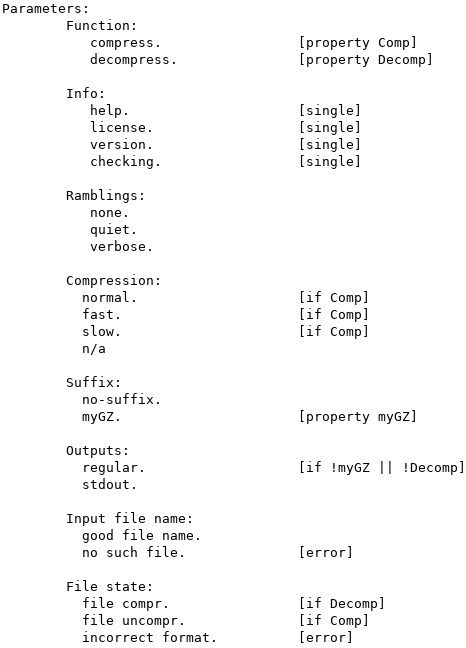
\includegraphics[width=3in,keepaspectratio]{tsl_input.png}
\caption{Category partition input format}
\label{fig:tsl_input}
\end{figure}

Combinatorial Interaction Testing -
\end{document}
